\appendix

\chapter{Annexes}


\section{Dictionnaires de données (datasets démo)}
\label{ann:a1-dictionnaires}

Cette annexe présente les champs nécessaires à la reproduction des prototypes, avec une description métier concise,
les types logique/technique, le rôle recommandé dans Power BI et les contraintes applicables. Les listes détaillées
sont volontairement reportées ici pour éviter les redondances dans le corps du texte.

\subsection{Passenger-Flow Map}
\begin{table}[ht]
\small
\setlength{\tabcolsep}{4pt}
\centering
\begin{tabularx}{\linewidth}{l X l l X X}
\toprule
Champ & Description & Type logique & Type technique & Rôle PBI & Contraintes\\
\midrule
EdgeId & Identifiant d’arête (ex. ENT1-G1). & identifiant & texte & Key (Do not summarize); Tooltip & Non nul; unique sur (EdgeId, Heure) \\
X1 & Abscisse source sur le plan SVG (px). & coordonnée & entier & Category (technique); Do not summarize & Non nul \\
Y1 & Ordonnée source sur le plan SVG (px). & coordonnée & entier & Category (technique); Do not summarize & Non nul \\
X2 & Abscisse cible sur le plan SVG (px). & coordonnée & entier & Category (technique); Do not summarize & Non nul \\
Y2 & Ordonnée cible sur le plan SVG (px). & coordonnée & entier & Category (technique); Do not summarize & Non nul \\
Passages & Volume de passagers sur l’arête pour l’heure donnée (personnes). & mesure (poids) & entier & Values (Sum); Tooltips & Non nul; valeur ≥ 0 \\
Heure & Heure civile agrégée (entier 0–23). & temps (discret) & entier & Category; Slicer & Domaine 0–23; participe à l’unicité avec EdgeId \\
Type & Nature du flux (Départ/Arrivée). & catégorie & texte & Legend; Category & Valeurs autorisées: \{Départ, Arrivée\} \\
\bottomrule
\end{tabularx}
\caption{Dictionnaire — Passenger-Flow Map}
\label{tab:a1-flows-compact}
\end{table}


\subsection{Sunburst budgétaire}
\begin{table}[ht]
\small
\setlength{\tabcolsep}{4pt}
\centering
\begin{tabularx}{\linewidth}{l X l l X X}
\toprule
Champ & Description & Type logique & Type technique & Rôle PBI & Contraintes\\
\midrule
Department & Niveau 1 de la hiérarchie budgétaire. & catégorie (N1) & texte & Category (Level 1) & Non nul; parent de SubDepartment \\
SubDepartment & Niveau 2 de la hiérarchie budgétaire. & catégorie (N2) & texte & Category (Level 2) & Non nul; enfant de Department; parent d’Account \\
Account & Niveau 3 (compte budgétaire). & catégorie (N3) & texte & Category (Level 3) & Non nul; enfant de SubDepartment \\
Amount & Montant affecté à l’élément hiérarchique (devise non spécifiée). & mesure (valeur) & entier & Values (Sum) & Aucune contrainte de signe imposée \\
\bottomrule
\end{tabularx}
\caption{Dictionnaire — Sunburst budgétaire}
\label{tab:a1-budget-compact}
\end{table}

\section{Fond de carte \& obstacles}
\label{ann:a2-fond}

Le prototype Passenger-Flow Map s'appuie sur un fond cartographique fixe et sur des obstacles modélisés en coordonnées normalisées. 
Pour éviter toute redondance dans le corps du texte, les éléments strictement techniques sont rassemblés ici.

\subsection{Schéma obstacles.json (extrait)}
Le fichier obstacles.json contient un tableau d'objets de la forme 
\{ id: string, points: number[2][] \}, où chaque paire \((x,y)\) est normalisée dans \([0,1]\). 
La conversion en pixels s'effectue par \(\hat x = x \cdot W\), \(\hat y = y \cdot H\) (largeur \(W\), hauteur \(H\) du canevas).

\begin{lstlisting}[language=json, basicstyle=\ttfamily\small, breaklines=true, breakatwhitespace=true, columns=fullflexible]
[
  {
    "id": "CHECKIN_DESK_1",
    "points": [
      [0.042, 0.386],
      [0.087, 0.386],
      [0.087, 0.656]
      ...
    ]
  },
  {
    "id": "BELT_1",
    "points": [
      [0.612, 0.366],
      [0.734, 0.366],
      [0.734, 0.409]
      ...
    ]
  }
  ...
]
\end{lstlisting}

\subsection{Schéma technique de superposition}
La superposition technique utilisée pour les démonstrations est fournie ci-dessous. 
Elle est dérivée des obstacles normalisés et permet d'aligner précisément les coordonnées des flux sur le fond.

\begin{figure}[h]
  \centering
  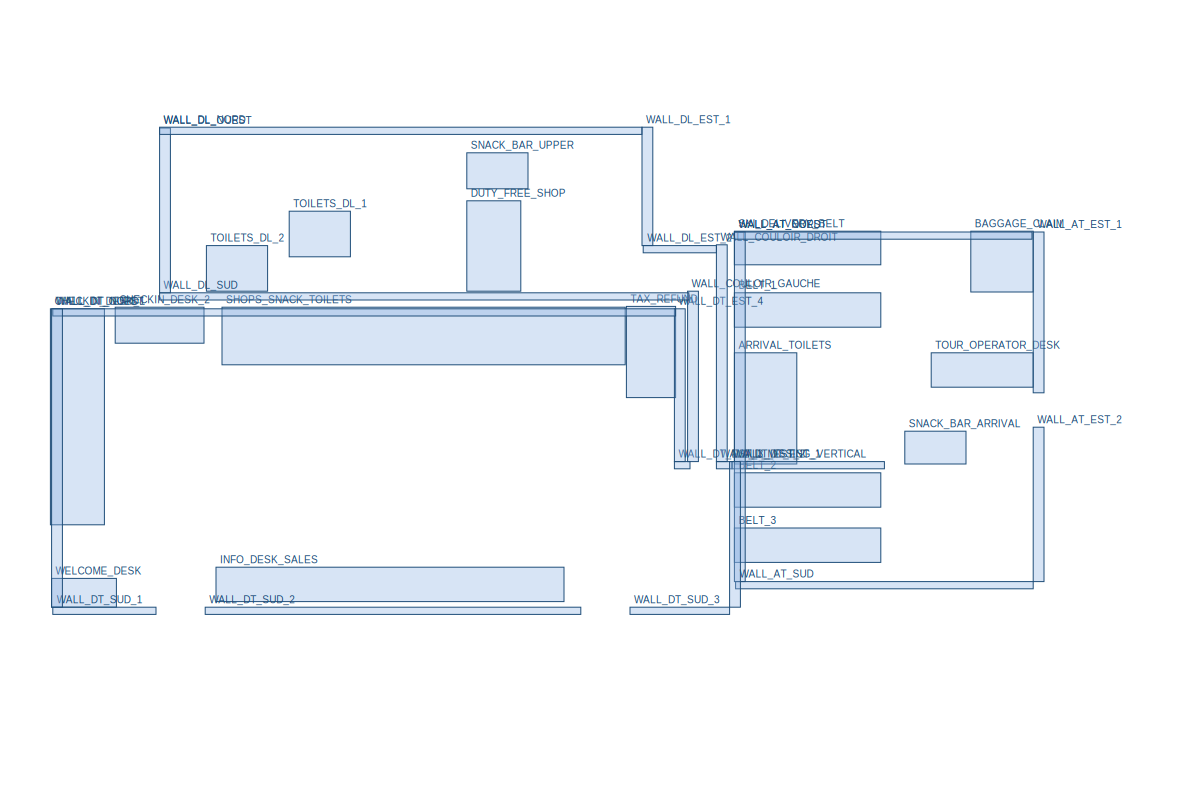
\includegraphics[width=.95\linewidth]{plan_overlay.png}
  \caption{Overlay technique généré à partir des obstacles normalisés.}
  \label{fig:a2-overlay}
\end{figure}

\subsection{Plan illustratif de l'aéroport (JPEG)}
Le fond illustratif utilisé pour les démonstrations (plan d’orientation de l’aéroport) est fourni pour référence.

\begin{figure}[h]
  \centering
  \includegraphics[width=.95\linewidth]{plan_interieur_gnb_hd.jpg}
  \caption{Plan illustratif de l'aéroport}
  \label{fig:a2-plan-jpeg}
\end{figure}

% =============================================================
% Annexe A3 — Tests et conformité (v4 — revue experte)
% -------------------------------------------------------------
\section{Tests et conformité}
\label{ann:a3-tests}

\subsection{Environnement et périmètre}
Après importation des fichiers, les tests techniques ont été réalisés sur Power~BI Desktop 
(canal classique) sous Windows~11, machine AMD Ryzen~7~9800X3D, 32~Go RAM, NVIDIA RTX~5080. 
Visuels évalués : \textit{Passenger-Flow Map} et \textit{Radial Sunburst Decomposition Tree} (version 2.0.0.0). 
Tailles mesurées des paquets \texttt{.pbiviz} (\textit{release} minifiée) : 
\textit{Radial Sunburst Decomposition Tree} \SI{37}{\kibi\byte} (\(\approx\) 37\,888~octets) ; 
\textit{Passenger-Flow Map} \SI{1006}{\kibi\byte} (\(\approx\) \SI{0.982}{\mebi\byte}). 
(Conversion effectuée depuis les valeurs «~Ko~» affichées par l’explorateur Windows vers KiB/MiB, norme IEC.) 
Jeux de données par défaut utilisés : \texttt{airport-flows-direct} et \texttt{sampleBudget}. 
Date des mesures : 05/08/2025 (cf. planning Waterfall du Chap.~3).

\begin{figure}[h]
  \centering
  \includegraphics[width=.95\linewidth]{Sunburst.png}
  \caption{Radial Sunburst Decomposition Tree — rendu sur dataset budgétaire de démonstration.}
\end{figure}

\begin{figure}[h]
  \centering
  \includegraphics[width=.95\linewidth]{Passenger-flow.png}
  \caption{Passenger-Flow Map — rendu sur dataset de flux passagers de démonstration.}
\end{figure}

\subsection{Protocole de mesure}
Les mesures de performance ont été saisies depuis l’Analyseur de performances de Power~BI, 
en relevant la durée «~Visual display (ms)~».  
\textbf{Critères projet (P95)} : \textit{Passenger-Flow Map} \(\leq\) 300~ms ; 
\textit{Radial Sunburst Decomposition Tree} \(\leq\) 100~ms (par interaction : chargement, drill, survol).

En complément des mesures techniques, une \textbf{revue experte formative} a été menée par la professeure référente 
(cf. Chap.~\ref{sec:validation-fonctionnelle}) afin d’évaluer la lisibilité, l’ergonomie de base et l’adéquation fonctionnelle.  
Cette revue constitue la seule source de retours qualitatifs ; aucun test utilisateur ou démonstration interne n’a été conduit.

\subsection{Résultats (synthèse)}
\begin{table}[h]
\scriptsize
\setlength{\tabcolsep}{3pt}
\centering
\begin{tabularx}{\linewidth}{l l r r r r c}
\toprule
\textbf{Visuel} & \textbf{Scénario} & \textbf{$n$} & \textbf{Moy (ms)} & \textbf{P95 (ms)} & \textbf{Seuil P95 (ms)} & \textbf{Conforme ?} \\
\midrule
Radial Sunburst Decomposition Tree & Global & 20 & 38.0 & 46.1 & 100 & Oui \\
Passenger-Flow Map & Global & 19 & 131.1 & 167.9 & 300 & Oui \\
\bottomrule
\end{tabularx}
\end{table}

\subsection{Distribution des temps (visualisations)}
\begin{figure}[h]
  \centering
  \includegraphics[width=.82\linewidth]{a4_sunburst_hist_v4.png}
  \caption{Radial Sunburst Decomposition Tree — histogramme des temps de cycle (ms).}
\end{figure}

\begin{figure}[h]
  \centering
  \includegraphics[width=.82\linewidth]{a4_map_hist_v4.png}
  \caption{Passenger-Flow Map — histogramme des temps de cycle (ms).}
\end{figure}

\subsection{Accessibilité (WCAG 2.2 — périmètre du projet)}
\begin{tabularx}{\linewidth}{l c X}
\toprule
\textbf{Critère} & \textbf{Statut} & \textbf{Preuve / commentaires} \\
\midrule
Navigation clavier (2.1.1) & Partiel & Non démontrable à partir des traces ; interactions testées principalement à la souris. À revérifier avec protocole clavier dédié. \\
Contraste (1.4.3) & À vérifier & Palette par défaut à contraste renforcé ; ratio à mesurer formellement sur les couples de couleurs configurés. \\
Internationalisation (3.1.x) & Conforme & Libellés fr-CH et en-US fournis ; bascule validée sur libellés de base. \\
\bottomrule
\end{tabularx}

\subsection{Sécurité et packaging}
\begin{tabularx}{\linewidth}{l X}
\toprule
\textbf{Vérification} & \textbf{État} \\
\midrule
Appels réseau sortants & Non utilisés (visuels autonomes, données locales Power BI). \\
\texttt{eval} / code dynamique & Non utilisé. \\
Stockage navigateur persistant & Non utilisé par défaut. \\
Taille du paquet \texttt{.pbiviz} & \textit{Radial Sunburst Decomposition Tree} \SI{37}{\kibi\byte} ; \textit{Passenger-Flow Map} \SI{1006}{\kibi\byte} (\(\approx\) \SI{0.982}{\mebi\byte}). \\
Seuil CI (artefact \texttt{.pbiviz}) & \(\leq\) \SI{1}{\mebi\byte} (= 1\,048\,576~octets). \\
Audit \texttt{--certification-audit} & À exécuter pour livraison : aucun blocant attendu sur ce périmètre. \\
\bottomrule
\end{tabularx}

\subsection{Couverture des tests unitaires}
\label{ann:a3-tests-coverage}

Les tests unitaires ont été exécutés avec Jest/ts-jest via \texttt{npm run test:cov} ; 
les rapports sont archivés dans \texttt{coverage/}.  
Le seuil CI retenu pour la couverture (déclarations) est fixé à \(\geq 70\%\). 
Les deux visuels satisfont ce seuil.

\begin{table}[H]\centering\small
\caption{Synthèse de couverture et d'exécution des tests}
\begin{tabular}{lrrrrrr}
\toprule
Visuel & \% Stmts & \% Branch & \% Funcs & \% Lines & Suites (ok/total) & Tests (ok/total) \\
\midrule
Radial Sunburst Decomposition Tree & 87.39 & 70.27 & 93.02 & 87.99 & 8/8  & 40/40 \\
Passenger-Flow Map                 & 80.64 & 76.30 & 75.45 & 80.66 & 19/19 & 51/51 \\
\bottomrule
\end{tabular}
\end{table}

En lecture rapide, le \textit{Sunburst} présente une couverture globalement élevée et homogène ; 
le \textit{Passenger-Flow Map} atteint des niveaux satisfaisants compte tenu de la part de logique graphique et d’interface.  
Ces résultats valident la robustesse des tests et la conformité au seuil CI sur le périmètre technique défini.

\section{Retours qualitatifs (revue experte)}
\label{ann:a4-retours}

Cette annexe synthétise les observations formulées lors de la revue experte réalisée 
par la professeure référente, en environnement Power~BI Service, 
sur les jeux de données de démonstration (\texttt{airport-flows-direct} et \texttt{sampleBudget}). 
Aucune autre session de test utilisateur ni démonstration interne n’a été conduite.

\subsection{Passenger-Flow Map}
\begin{itemize}[nosep]
  \item \textbf{Lisibilité des flux principaux} : claire dès le premier coup d’œil. Suggestion d’ajouter une variation d’épaisseur des traits par zone pour renforcer la hiérarchie visuelle.
  \item \textbf{Carte de chaleur} : pertinente pour repérer les zones d’affluence, mais l’échantillon de données de démonstration ne permet pas de tester pleinement son potentiel.
  \item \textbf{Légende et couleurs} : ajout d’une légende jugé utile ; possibilité de définir manuellement les paliers de couleur recommandée.
\end{itemize}

\subsection{Sunburst hiérarchique}
\begin{itemize}[nosep]
  \item \textbf{Hiérarchie et proportions} : compréhension immédiate.
  \item \textbf{Navigation} : drill-down, drill-up et fil d’Ariane jugés naturels et faciles à utiliser.
  \item \textbf{KPI central} : non indispensable mais pas gênant ; peut rester optionnel.
\end{itemize}

\subsection{Synthèse}
La revue experte conclut que les deux visuels répondent à leurs objectifs métier initiaux.  
La \textit{Passenger-Flow Map} apparaît comme un composant spécialisé, 
avec des pistes d’amélioration sur la personnalisation visuelle et la clarté des légendes.  
Le \textit{Sunburst} se distingue par sa polyvalence et son adaptabilité à différents contextes hiérarchiques.



\section{Procédure développeur}
\label{ann:a5-dev}

\subsection{Prérequis (environnement)}
\begin{tabularx}{\linewidth}{l X}
\toprule
\textbf{Composant} & \textbf{Version / Remarque} \\
\midrule
OS & Windows 11 (64-bit) \\
Power BI Desktop & Canal classique (build courant) \\
Node.js & 22.x (LTS) \\
npm & 10/11 \\
Power BI Visual Tools (pbiviz) & 6.1.3 \\
\bottomrule
\end{tabularx}

\subsection{Arborescence de référence}
\begin{lstlisting}[basicstyle=\ttfamily\small]
/ (racine du dépot)
  src/                  # sources TypeScript du visuel
  assets/               # ressources statiques (icones, styles)
  tests/                # tests unitaires Jest (optionnel)
  dist/                 # artefacts .pbiviz (généré)
  coverage/             # rapports de couverture (généré)
  scripts/              # scripts internes (signature, etc.)
    make_signing_keys.ps1
    make_signing_keys.sh
    openssl.cnf         # config locale si nécessaire (Windows)
  capabilities.json
  pbiviz.json
  package.json
  tsconfig.json
  .eslintrc.cjs
  .gitignore
\end{lstlisting}

\subsection{\texttt{tsconfig.json} (inclure les \texttt{.d.ts})}
\begin{lstlisting}[language=json,basicstyle=\ttfamily\small,breaklines=true,columns=fullflexible]
{
  "compilerOptions": {
    "allowJs": false,
    "emitDecoratorMetadata": true,
    "experimentalDecorators": true,
    "target": "es2022",
    "sourceMap": true,
    "outDir": "./.tmp/build/",
    "moduleResolution": "node",
    "declaration": true,
    "lib": ["es2022", "dom"]
  },
  "files": ["./src/visual.ts"],
  "include": ["src/**/*.ts", "src/**/*.tsx", "src/**/*.d.ts"],
  "exclude": ["node_modules", "dist", ".tmp", "coverage"]
}
\end{lstlisting}

\subsection{Scripts NPM (référence)}
\begin{lstlisting}[language=json,basicstyle=\ttfamily\small,breaklines=true,columns=fullflexible]
{
  "scripts": {
    "lint": "eslint . --ext .ts,.tsx -f stylish",
    "lint:ci": "eslint . --ext .ts,.tsx -f unix --max-warnings=0",
    "test": "jest --ci",
    "test:cov": "jest --ci --coverage --passWithNoTests --coverageReporters=json-summary --coverageReporters=text --coverageReporters=lcov",
    "start": "pbiviz start",
    "build": "pbiviz package"
  }
}
\end{lstlisting}

\subsection{Toolchain de build (devDependencies minimales)}
\begin{itemize}
  \item \texttt{webpack}, \texttt{webpack-cli}, \texttt{typescript}, \texttt{ts-loader}
  \item \texttt{css-loader}, \texttt{json-loader}, \texttt{less}, \texttt{less-loader}
  \item Qualité/tests : \texttt{eslint}, \texttt{@typescript-eslint/\{parser,eslint-plugin\}}, \texttt{jest}, \texttt{ts-jest}
\end{itemize}

\subsection{\texttt{.gitignore} (extraits pertinents)}
\begin{lstlisting}[basicstyle=\ttfamily\small]
node_modules/
dist/
coverage/
.tmp/
webpack.statistics*.html

# Clés/certificats internes (ne pas versionner)
scripts/ecrins-root.key
scripts/ecrins-root.crt
scripts/_codesign.key
scripts/_codesign.crt
*.p7s
\end{lstlisting}

\subsection{Démarrage local (dev)}
1) \texttt{npm ci}. 2) \texttt{pbiviz start}. Au premier lancement, installer le certificat HTTPS proposé par \texttt{pbiviz} (magasin « Autorités de certification racines de confiance »). 3) Power BI Desktop~\(\rightarrow\) Options~\(\rightarrow\) Sécurité~: activer le mode développeur. Le visuel Developer apparaît dans le ruban.

\subsection{Packaging local (\texttt{.pbiviz})}
Exécuter \texttt{pbiviz package --certification-audit}. Conserver le \texttt{packaging.log}. Vérifier l’incrément de version dans \texttt{pbiviz.json} (\(MAJOR.MINOR.PATCH\)). La CI orchestre les mêmes commandes (chap.~\ref{chap:industrialisation}).

\subsection{Contrôles rapides (QA)}
Lint \& tests~: \texttt{npm run lint} \& \texttt{npm test} ; taille du paquet \(\leq\)~1~MiB ; audit sans bloquant ; démarrage Desktop OK.
\section{Publication dans le magasin organisationnel : vérifications préalables et mode opératoire}
\label{ann:org-store-procedure}

\subsection{Pré-requis côté administrateur (mise à jour)}
Dossier attendu pour la revue :
\begin{itemize}
  \item Paquet \texttt{.pbiviz}
  \item Empreinte \texttt{.pbiviz.sha256}
  \item Journal d’audit (\texttt{packaging.log})
  \item Signature \texttt{.pbiviz.p7s} (si signature interne activée)
  \item Référence de version (tag Git) et changelog
  \item Certificat racine interne (\texttt{scripts/ecrins-root.crt}) pour vérification locale
\end{itemize}

\subsection{Vérification d’intégrité (SHA-256)}
\textbf{Linux/macOS}
\begin{verbatim}
sha256sum -c MonVisuel.pbiviz.sha256
# "OK" confirme la correspondance empreinte/fichier
\end{verbatim}
\textbf{Windows PowerShell}
\begin{verbatim}
Get-FileHash .\MonVisuel.pbiviz -Algorithm SHA256
# Comparer au contenu de MonVisuel.pbiviz.sha256
\end{verbatim}

\subsection{Vérification de la signature (si activée)}
\textbf{Linux/macOS}
\begin{verbatim}
openssl smime -verify -binary \
  -in MonVisuel.pbiviz.p7s -inform DER \
  -content MonVisuel.pbiviz \
  -CAfile scripts/ecrins-root.crt -purpose any -out /dev/null
# Code retour 0 : signature valide et chaîne approuvée
\end{verbatim}
\textbf{Windows}
Utiliser OpenSSL pour Windows avec la commande ci-dessus, ou importer la racine interne
dans le magasin d’autorités approuvées et utiliser l’outil interne.
% =============================================================
% A.6 — Activer la signature interne (parcours simple)
% =============================================================
\section{Activer la signature interne (parcours simple)}
\label{ann:signature-procedure}

\subsection*{Objet et périmètre}
Mise en place simple d’une signature interne pour les paquets \texttt{.pbiviz}. Optionnelle : sans activation, la vérification se limite à l’empreinte d’intégrité (SHA-256).

\subsection*{Étape 0 — Prérequis}
Installer OpenSSL.\\
\textbf{Windows (winget)} : \verb|winget install -e --id ShiningLight.OpenSSL.Light|\\
\textbf{macOS} : \verb|brew install openssl| \quad \\
\textbf{Linux (Debian/Ubuntu)} : \verb|sudo apt update && sudo apt install -y openssl|

\noindent\textit{Note (Windows).} Certaines distributions OpenSSL référencent un \texttt{OPENSSLDIR} non présent localement. Pour éviter les erreurs, fournir un fichier local \texttt{scripts/openssl.cnf} et, si nécessaire, le référencer via \texttt{-config}.

\begin{lstlisting}[basicstyle=\ttfamily\small]
openssl_conf = openssl_init
[openssl_init]
providers = provider_sect
[provider_sect]
default = default_sect
[default_sect]
activate = 1
[req]
distinguished_name = dn
[dn]
\end{lstlisting}

\subsection*{Étape 1 — Générer la racine et le certificat (scripts locaux)}
Créer \texttt{scripts/make\_signing\_keys.ps1} (Windows) ou \texttt{scripts/make\_signing\_keys.sh} (macOS/Linux), puis exécuter. Fichiers produits : \texttt{scripts/ecrins-root.crt},\\\texttt{scripts/ecrins-root.key}, \\\texttt{scripts/ecrins-codesign.crt}, \texttt{scripts/ecrins-codesign.key}. Une passphrase est affichée ; la conserver en lieu sûr.

\textbf{PowerShell (Windows) — \texttt{scripts/make\_signing\_keys.ps1}}
\begin{lstlisting}[basicstyle=\ttfamily\small,breaklines=true,columns=fullflexible]
param(
  [string]$Country="CH", [string]$Org="ECRINS SA",
  [string]$RootCN="ECRINS Visuals Root CA",
  [string]$CodeCN="ECRINS Visuals Code Signing",
  [int]$RootDays=3650, [int]$CodeDays=1095
)
$ErrorActionPreference = "Stop"
function New-RandBase64([int]$n=32){
  $b=New-Object byte[] $n
  [Security.Cryptography.RandomNumberGenerator]::Create().GetBytes($b)
  [Convert]::ToBase64String($b)
}
if(-not(Get-Command openssl -ErrorAction SilentlyContinue)){
  Write-Error "OpenSSL indisponible"
}
New-Item -ItemType Directory -Force -Path "scripts" | Out-Null
Push-Location scripts
@"
openssl_conf = openssl_init
[openssl_init]
providers = provider_sect
[provider_sect]
default = default_sect
[default_sect]
activate = 1
[req]
distinguished_name = dn
[dn]
"@ | Set-Content -Encoding ascii openssl.cnf
$config = (Resolve-Path .\openssl.cnf).Path
$rootPass=New-RandBase64; $codePass=New-RandBase64
# Racine
openssl genpkey -algorithm RSA -out ecrins-root.key -aes-256-cbc -pass pass:$rootPass -pkeyopt rsa_keygen_bits:4096
openssl req -x509 -new -key ecrins-root.key -passin pass:$rootPass -sha256 -days $RootDays -subj "/C=$Country/O=$Org/CN=$RootCN" -config "$config" -out ecrins-root.crt
# Signature
openssl genpkey -algorithm RSA -out ecrins-codesign.key -aes-256-cbc -pass pass:$codePass -pkeyopt rsa_keygen_bits:3072
openssl req -new -key ecrins-codesign.key -passin pass:$codePass -subj "/C=$Country/O=$Org/CN=$CodeCN" -config "$config" -out ecrins-codesign.csr
@"
basicConstraints=CA:FALSE
keyUsage=digitalSignature
extendedKeyUsage=codeSigning
subjectKeyIdentifier=hash
authorityKeyIdentifier=keyid,issuer
"@ | Set-Content -Encoding ascii codesign.ext
openssl x509 -req -in ecrins-codesign.csr -CA ecrins-root.crt -CAkey ecrins-root.key -passin pass:$rootPass -CAcreateserial -out ecrins-codesign.crt -days $CodeDays -sha256 -extfile codesign.ext
Write-Host "`nSecrets à créer : ECRINS_CODESIGN_CRT / ECRINS_CODESIGN_KEY / ECRINS_CODESIGN_PASS"
Write-Host ("ECRINS_CODESIGN_PASS = {0}" -f $codePass)
Pop-Location
\end{lstlisting}

\textbf{Bash (macOS/Linux) — \texttt{scripts/make\_signing\_keys.sh}}
\begin{lstlisting}[basicstyle=\ttfamily\small,breaklines=true,columns=fullflexible]
#!/usr/bin/env bash
set -euo pipefail
C="${1:-CH}"; O="${2:-ECRINS SA}"
ROOT_CN="${3:-ECRINS Visuals Root CA}"
CODE_CN="${4:-ECRINS Visuals Code Signing}"
ROOT_DAYS="${5:-3650}"; CODE_DAYS="${6:-1095}"
mkdir -p scripts && cd scripts
code_pass="$(openssl rand -base64 32)"
root_pass="$(openssl rand -base64 32)"
cat > openssl.cnf <<'CNF'
openssl_conf = openssl_init
[openssl_init]
providers = provider_sect
[provider_sect]
default = default_sect
[default_sect]
activate = 1
[req]
distinguished_name = dn
[dn]
CNF
# Racine
openssl genpkey -algorithm RSA -out ecrins-root.key -aes-256-cbc -pass pass:"$root_pass" -pkeyopt rsa_keygen_bits:4096
openssl req -x509 -new -key ecrins-root.key -passin pass:"$root_pass" -sha256 -days "$ROOT_DAYS" -subj "/C=$C/O=$O/CN=$ROOT_CN" -config openssl.cnf -out ecrins-root.crt
# Signature
openssl genpkey -algorithm RSA -out ecrins-codesign.key -aes-256-cbc -pass pass:"$code_pass" -pkeyopt rsa_keygen_bits:3072
openssl req -new -key ecrins-codesign.key -passin pass:"$code_pass" -subj "/C=$C/O=$O/CN=$CODE_CN" -config openssl.cnf -out ecrins-codesign.csr
cat > codesign.ext <<'EOF'
basicConstraints=CA:FALSE
keyUsage=digitalSignature
extendedKeyUsage=codeSigning
subjectKeyIdentifier=hash
authorityKeyIdentifier=keyid,issuer
EOF
openssl x509 -req -in ecrins-codesign.csr -CA ecrins-root.crt -CAkey ecrins-root.key -passin pass:"$root_pass" -CAcreateserial -out ecrins-codesign.crt -days "$CODE_DAYS" -sha256 -extfile codesign.ext
echo "ECRINS_CODESIGN_PASS = $code_pass"
\end{lstlisting}

\noindent\textbf{Exécution.}
\begin{verbatim}
# Windows
pwsh -File scripts/make_signing_keys.ps1

# macOS/Linux
chmod +x scripts/make_signing_keys.sh
./scripts/make_signing_keys.sh
\end{verbatim}

\subsection*{Étape 2 — Créer les secrets GitHub (noms exacts)}
Dans \textit{Settings} → \textit{Secrets and variables} → \textit{Actions} → \textit{New repository secret}.\\
\texttt{ECRINS\_CODESIGN\_CRT} → contenu de \texttt{scripts/ecrins-codesign.crt}\\
\texttt{ECRINS\_CODESIGN\_KEY} → contenu de \texttt{scripts/ecrins-codesign.key}\\
\texttt{ECRINS\_CODESIGN\_PASS} → passphrase affichée

\subsection*{Étape 3 — Lancer une release}
Créer un tag \texttt{vX.Y.Z} et le pousser. La CI publie : \texttt{.pbiviz}, \texttt{.pbiviz.sha256}, \texttt{packaging.log} et, si secrets présents, \texttt{.pbiviz.p7s}. Voir l’annexe~\ref{ann:org-store-procedure} pour la vérification d’intégrité et de signature.

\subsection*{Sécurité}
Ne pas versionner \texttt{scripts/ecrins-root.key} ni \texttt{scripts/ecrins-root.crt}. Restreindre l’accès aux secrets GitHub et planifier leur rotation.
